\tikzset{->-/.style={decoration={
  markings,
  mark=at position .5 with {\arrow{>}}},postaction={decorate}}}

  \tikzset{-<-/.style={decoration={
  markings,
  mark=at position .5 with {\arrow{<}}},postaction={decorate}}}

\subsection{Overview}
 The network model we use is exactly as in \citet{eisenberg2001systemic} and \citet{glasserman2015likely}. The nodes of the network are all US domestic financial institutions. The connections between nodes are defined by institutions borrowing from and lending to one another. There is a link from node $i$ to node $j$ if $i$ has any payment obligations towards node $j$. In addition to lending to one another, nodes can borrow and lend to the rest of the domestic and global economy. These assets and liabilities are termed as \textit{outside} the financial system. In our application, the \textit{outside} sector is comprised of domestic and foreign non-financial institutions, governments, and households, as well as foreign financial institutions.

Figure \ref{fig:networkExample} shows an example of a simple network, taken from \citet{glasserman2015likely}. The four arrows originating in the central node and pointing to the four peripheral nodes show that the central node owes $10$ to each of the peripheral nodes. The four peripheral nodes have no borrowing or lending among themselves. For this network, we say that the central node has \textit{inside liabilities }of $40$, while each of the peripheral nodes has \textit{inside assets} of $10$. In practice, we find that inside assets and liabilities for US financial institutions are primarily composed of deposits, loans and securities lending transactions.

%\begin{figure}[h!]
%\par
%\begin{center}
%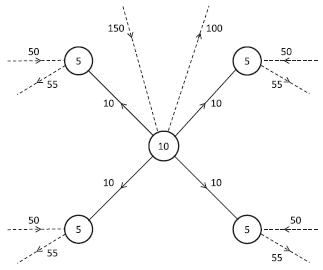
\includegraphics[width=10cm]{fig1_networkExample.png} %
%\end{center}
%\end{figure}

\begin{figure}
\par
\begin{center}
\begin{tikzpicture}[xscale=.5, yscale=.5]

\draw (5, 5) circle [radius=1];
\node at (5,5) {$10$};
\draw (10, 10) circle [radius=1];
\node at (10,10) {$5$};
\draw (10, 0) circle [radius=1];
\node at (10,0) {$5$};
\draw (0, 10) circle [radius=1];
\node at (0,10) {$5$};
\draw (0, 0) circle [radius=1];
\node at (0,0) {$5$};

\draw[dashed, -<-] (-1, 10) -- (-4, 10);
\draw[dashed, ->-] (-.7071, 9.2929) -- (-2.82843, 7.171573);
\node [below] at (-2.5, 10) {\footnotesize $50$};
\node [right] at (-1.76777, 8.232233) {\footnotesize $55$};

\draw[dashed, -<-] (-1, 0) -- (-4, 0);
\draw[dashed, ->-] (-.7071, -.7071) -- (-2.82843, -2.82843);
\node [below] at (-2.5, 0) {\footnotesize $50$};
\node [right] at (-1.76777, -1.76777) {\footnotesize $55$};

\draw[dashed, -<-] (11, 10) -- (14, 10);
\draw[dashed, ->-] (10.7071, 9.2929) -- (12.82843, 7.171573);
\node [below] at (12.5, 10) {\footnotesize $50$};
\node [left] at (11.76777, 8.232233) {\footnotesize $55$};

\draw[dashed, -<-] (11, 0) -- (14, 0);
\draw[dashed, ->-] (10.7071, -.7071) -- (12.82843, -2.82843);
\node [below] at (12.5, 0) {\footnotesize $50$};
\node [left] at (11.76777, -1.76777) {\footnotesize $55$};

\draw[dashed, -<-] (4.2929, 5.7071) -- (3.75, 12);
\draw[->-] (4.2929, 5.7071) -- (.7071, 9.2929);
\draw[dashed,  ->-] (5.7071, 5.7071) -- (6.5, 12);
\draw[->-] (5.7071, 5.7071) -- (9.2929, 9.2929);
\draw[->-] (4.2929, 4.2929) -- (.7071, .7071);
\draw[->-] (5.7071, 4.2929) -- (9.2929, .7071);
\node [left] at (4, 9) {\footnotesize $150$};
\node [left] at (6, 9) {\footnotesize $100$};
\node [left] at (3, 7) {\footnotesize $10$};
\node [right] at (7, 7) {\footnotesize $10$};
\node [left] at (3, 3) {\footnotesize $10$};
\node [right] at (7, 3) {\footnotesize $10$};
\end{tikzpicture}

\end{center}
\caption{\textbf{A simple network}. Nodes are financial institutions. There is a connection from node $i$ to node $j$ if $i$ is a net borrower from $j$. The dashed lines show connections to the outside sector.}
\label{fig:networkExample}\vspace{.3in}
\end{figure}


In addition to its claims inside the network, the central node has lent $150$ and has borrowed $100$ from the outside sector, depicted by the dashed lines with arrows going into and out of the central node. We refer to positive claims with respect to the outside sector as \textit{outside assets} and to negative claims as \textit{outside liabilities}. Outside assets typically consist of securities, loans to firms and households (including mortgages), and public debt. Outside liabilities mostly involve deposits and lines of credit.

The difference between all assets and all liabilities gives each node's net worth. The central node has a net worth of $10$, shown inside the circle that represents the node.  Each of the peripheral nodes has outside assets of $50$, outside liabilities of $55$ and an inside asset of $10$ with respect to the central node, for a net worth of $5$.

\subsection{Shocks and Propagation}

The shocks we consider are exogenous reductions in the value of outside assets. Therefore, all initial losses always originate outside the network. One example of such a shock is an increase in defaults for residential mortgages held by financial institutions.

For sufficiently high initial losses in outside assets, some nodes in the network will be unable to pay their creditors in full. When this happens, all debts for the defaulting node (including those outside the network) are written down pro rata and creditors receive only a fraction of their promised payments. Note that under a pro rata allocation, a node defaults on either all of its creditors or none of them. When creditors for some node are not paid in full, they may themselves be unable to pay their own creditors, and so on. Initial losses thus get transmitted inside the network through this ``domino'' effect. We do not include in our analysis any liquidity or equity injections, and only net claims between two nodes are assumed to be of relevance (as opposed to gross positions). In addition, nodes do not renegotiate claims, even if it may be mutually beneficial to do so.

As a numerical example, consider what happens when the outside assets of the central node in Figure \ref{fig:networkExample} receive a shock of size $80$. Outside assets for the central node decrease from $150$ to $70$. Total liabilities are initially $140$. After the shock, under a pro rata allocation, only $50$ percent of each liability is repaid as the central node only has $70$ remaining in assets. Each of the peripheral nodes receives $5$ from the central node, just enough to balance their assets and liabilities. A shock to the outside assets of the central node of magnitude greater than $80$ would reduce the value of assets for peripheral nodes below the value of their liabilities. In this case, the peripheral nodes would default on their creditors. In this case, the central node has created contagion to the peripheral nodes through network contagion. The peripheral nodes default even though none of their outside assets were affected by the initial shock.

\subsection{The Disconnected Network}

To quantify the amplification of losses stemming from the network structure --as opposed to the initial losses from exogenous shock to outside assets-- we compare expected losses for the system (the network plus the outside sector) to the losses in a hypothetical system in which all connections inside the network have been severed. Both networks are subject to the same distribution of exogenous shocks to outside assets, and to no other shocks. We create this hypothetical \textit{disconnected} system by removing all connections between nodes inside the original network but keeping the links with the outside sector intact. We also assume the net worth at each node remains unchanged by creating, for each node, a fictitious claim to the outside sector equal in value to the net value of all the connections that were removed. Depending on the sign of the net value of removed connections, the new fictitious claim can be an asset or a liability. If it is an asset, we assume it is not subject to the shocks to outside assets to keep the set of assets initially shocked identical to that of the original network. If the new fictitious claim is a liability, we assume it has the same priority as all other liabilities. In case of default, the new fictitious liability gets haircut pro rata just like all other non-fictitious liabilities, and any ``losses'' imposed on that obligation are counted towards the value of total system losses. Figure \ref{fig:disconnectedNetwork} shows the disconnected version of network displayed in Figure \ref{fig:networkExample}.

\begin{figure}
\par
\begin{center}
\begin{tikzpicture}[xscale=.5, yscale=.5]

\draw (5, 5) circle [radius=1];
\node at (5,5) {$10$};
\draw (10, 10) circle [radius=1];
\node at (10,10) {$5$};
\draw (10, 0) circle [radius=1];
\node at (10,0) {$5$};
\draw (0, 10) circle [radius=1];
\node at (0,10) {$5$};
\draw (0, 0) circle [radius=1];
\node at (0,0) {$5$};

\draw[dashed, -<-] (-1, 10) -- (-4, 10);
\draw[dotted, -<-] (-1, 10) -- (-4, 11.5);
\draw[dashed, ->-] (-.7071, 9.2929) -- (-2.82843, 7.171573);
\node [below] at (-2.5, 10) {\footnotesize $50$};
\node [right] at (-1.76777, 8.232233) {\footnotesize $55$};
\node [above] at (-2.5, 11) {\footnotesize $10$};

\draw[dashed, -<-] (-1, 0) -- (-4, 0);
\draw[dotted, -<-] (-1, 0) -- (-4, 1.5);
\draw[dashed, ->-] (-.7071, -.7071) -- (-2.82843, -2.82843);
\node [below] at (-2.5, 0) {\footnotesize $50$};
\node [right] at (-1.76777, -1.76777) {\footnotesize $55$};
\node [above] at (-2.5, 1) {\footnotesize $10$};

\draw[dashed, -<-] (11, 10) -- (14, 10);
\draw[dotted, -<-] (11, 10) -- (14, 11.5);
\draw[dashed, ->-] (10.7071, 9.2929) -- (12.82843, 7.171573);
\node [below] at (12.5, 10) {\footnotesize $50$};
\node [above] at (12.5, 11) {\footnotesize $10$};
\node [left] at (11.76777, 8.232233) {\footnotesize $55$};

\draw[dashed, -<-] (11, 0) -- (14, 0);
\draw[dotted, -<-] (11, 0) -- (14, 1.5);
\draw[dashed, ->-] (10.7071, -.7071) -- (12.82843, -2.82843);AH
\node [below] at (12.5, 0) {\footnotesize $50$};
\node [above] at (12.5, 1) {\footnotesize $10$};
\node [left] at (11.76777, -1.76777) {\footnotesize $55$};

\draw[dashed, -<-] (4.2929, 5.7071) -- (4, 12);
\draw[dashed, ->-] (5.7071, 5.7071) -- (6, 12);
\draw[dotted, ->-] (5.7071, 5.7071) -- (8, 12);
\node [left] at (4.25, 9) {\footnotesize $150$};
\node [left] at (6, 9) {\footnotesize $100$};
\node [right] at (6.5, 8) {\footnotesize $40$};

\end{tikzpicture}

\end{center}
\caption{\textbf{A Simple Disconnected Network}. The disconnected version of 
the networks in Figure \ref{fig:networkExample} are obtained by
removing all connections between nodes inside the original network but
keeping the links with the outside sector intact. Net
worth remains unchanged by creating fictitious outside assets or liabilities. Dashed lines indicate actual balance sheet assets and liabilities, and dotted lines indicate fictitious assets from or liabilities to the outside sector.}
\label{fig:disconnectedNetwork}\vspace{.3in}
\end{figure}

\subsection{An Upper Bound on Network Spillovers}

We are interested in whether the expected system losses in our real-world, interconnected system are substantially greater than those in the hypothetical \textit{disconnected} system, where node connections have been excised. We define $R$ to be the ratio of expected losses for the actual network to the expected losses in the disconnected network. That is, if $L$ denotes total system losses,

\begin{equation}
R=\frac{E(L_{\text{Actual}})}{E(L_\text{Disconnected})}
\end{equation}


The value of $R$ gives the relative magnitude of additional losses imposed on the system because of the interconnected structure of the network - to wit, network effect losses. With perfect information on the bilateral claims in the system, this ratio could be calculated exactly in response to a variety of shocks by using the \citet{eisenberg2001systemic} algorithm to compute the set of node payments that `clear' the system (i.e. follow the system's rules of limited liability and pro rata allocation). In the United States financial system, detailed and publicly-available data on bilateral obligations between financial firms does not exist. 

The main result in \citet{glasserman2015likely} is that a useful upper-bound on $R$ can be derived without any information on the makeup of each node's bilateral claims. We call this upper-bound $B$. If the tails of the distribution of exogenous shocks to outside assets are not too fat-tailed, then $B$ can be calculated using node-specific information only\footnote{More technically, we consider shocks that have an \textquotedblleft increasing failure rate" (IFR). A random variable with distribution function  $G\left( x\right) $ and density $g\left( x\right) $ is said to have an IFR if $g\left( x\right) /(1-G\left( x)\right) $ is an increasing function of $x$ . This family encompasses the normal, exponential, and uniform distributions. There are no restrictions on the correlation structure of shocks.  \par In addition, the joint distribution of potential shocks is assumed to be invariant to scale (homogeneous in assets). For example, if total assets of a node double, expected losses are assumed to also double.}. \citet{glasserman2015likely} show that $B$ depends only on each node's total outside assets $c$, each firm's probability of default due to direct shocks to outside assets $\delta$, and the maximum \textit{liability connectivity} among nodes in the system $\beta^+$. Each node's liability connectivity is defined as its ratio of inside liabilities to total liabilities.

\citet{glasserman2015likely} show that

\begin{equation} \label{eq:B}
B=1+\frac{1}{(1-\beta ^{+})}\frac{\sum_{i \in S} {\delta _{i}c_{i}}}{\sum_{i \in S}{c_{i}}},
\end{equation}

\begin{eqnarray*}
\delta _{i} &:&\text{probability of default from outside shocks for node }i, \\
c_{i} &:&\text{the dollar value of outside assets for node }i, \\
\beta ^{+} &:&\text{maximum liability connectivity, i.e., }\beta^{+}=\max_{i \in S}\beta _{i}\text{, with } \beta_i=\text{the fraction of } \\
&& \text{firm i's liabilities held by other nodes in the networks}, \\
S &:&\text{Set of financial institution nodes within the network.}
\end{eqnarray*}%

The upper bound $B$ for network spillovers is increasing in the maximum financial connectivity of the system, $\beta ^{+}$, and in the quantity $\sum {\delta _{i}c_{i}}/\sum {c_{i}}$, most-easily interpretable as a weighted average probability of default for the system (with each firm's weight given by its share of total outside assets). When $\beta ^{+}$ is close to $1$, aggregate financial connectivity is high and any initial shock to outside assets has the potential to be transmitted broadly across the network. In contrast, when $\beta ^{+}$ is close to zero, any initial shock dissipates quickly and expected losses should be similar to those in a truly disconnected network.

For most systems calibrated to real-world data, previous studies have found that the upper bound $B$ is small. For example, picking $\beta ^{+}=0.8$ and $\delta _{i}=1$ percent for all nodes $i$, we get $B=1+0.01/(1-0.8)=1.05$. This means that the connected system has expected losses that are at most $5$ percent larger than those in the system of isolated nodes. In their example exercise, \citet{glasserman2015likely} find an even smaller upper bound of $1.0175$ for European banks using data from the the 2011 European Banking Authority stress test.

\subsection{The Network Vulnerability Index}

We define the \emph{Network Vulnerability Index} (NVI) to be the upper bound on the magnitude of additional expected losses created in the system by network spillovers, expressed as a share of expected disconnected system:

\begin{equation} \label{eq:NVI}
NVI=\left( B-1\right) = \frac{1}{(1-\beta ^{+})}\frac{\sum {\delta _{i}c_{i}}}{\sum {c_{i}}}.
\end{equation}

Being an upper bound, the $NVI$ is most useful when its value is small, since the model then clearly indicates low vulnerability to potential network spillovers. When the index is large it is less informative. In this case, the true value of potential network spillovers could be as large as the upper bound or as low as zero, as dictated by the bilateral claims between nodes. The model does not produce any additional information that can help pinpoint the true value of network spillovers within that the range $\left[ 0,NVI\right] $. As an extreme, when the $NVI$ is equal to infinity, it provides no information\footnote{In this section, we have used the words ``small'' and ``large'' to characterize different levels of the $NVI$ without being explicit about their meaning. This was a deliberate choice, since the model provides no welfare analysis and no other indication on how to evaluate the overall magnitude of the $NVI$. In short, the burden of interpreting what constitutes small or large values for the $NVI$ is the policymaker's.}.

\subsection{A Firm-Specific Risk Measure: The `Contagion Index'}

\citet{glasserman2015likely} also presents a firm-specific measure of the potential to cause contagion, which they term a firm's `contagion index'. For a wide family of shocks, the index is defined as 

\[\text{contagion index} = w_i \beta_i \lambda_i\]

\noindent where $w_i$ is a firm's net worth, $\beta_i$ is liability connectivity as in equation \ref{eq:NVI}, and $\lambda_i=\frac{c_i}{w_i}$ is the leverage of firm $i$'s outside assets. 

Given that the magnitude of exogenous shocks to outside assets in the model is bounded by each firm's actul quantity of outside assets, the contagion index calculates the total payment shortfall that a firm could potentially pass on to other nodes following a shock to its own outside assets. \citet{glasserman2015likely} show that an outside asset shock to node $i$ cannot possibly cause default to node $j$ if node $j$'s net worth is greater than node $i$'s contagion index. They also show that the \textit{probability} of node $j$ defaulting solely because of a shock to node $i$'s assets \textit{must} be less than the probability of node $j$ defaulting from a shock to its own assets if $i$'s contagion index is less than $j$'s quantity of outside assets, $c_j$\footnote{The bounds derived by \citet{glasserman2015likely} are actually stronger than this - applying to the probability of node $i$ causing default through contagion to a given \textit{group} of firms.}.